\documentclass{llncs}

\usepackage{graphicx}
\usepackage{mwe}
\usepackage{subfig}
\usepackage{amsmath}
\usepackage{amssymb}
\usepackage{rotating}

\begin{document}

\title{Numerical modelling of physical systems}
\author{ Pawel Czyz }

\authorrunning{Pawel Czyz}

\institute{St. Hugh's College, University of Oxford,\\
Margaret Road, Oxford OX2 6LE, UK\\
\email{pawel.czyz@st-hughs.ox.ac.uk}}

\maketitle

\begin{abstract}
We present a new Python library enabling scientist to write accurate and effective numerical simulations. We investigate it's accuracy in a range of physical
models, as Lorentz attractor and quantum harmonic oscillator.

\keywords{numerical modelling, Runge-Kutta, Numerov, chaos}
\end{abstract}

\section{Introduction}

\section{Numerical methods}
\subsection{Runge-Kutta method}
\subsection{Numerov's method}

\section{Models of physical systems}
\subsection{Classical harmonic oscillator}
\subsection{Lorentz attractor}
\subsection{Quantum harmonic oscillator}

\section{Conclusions}

\begin{figure}
\centering
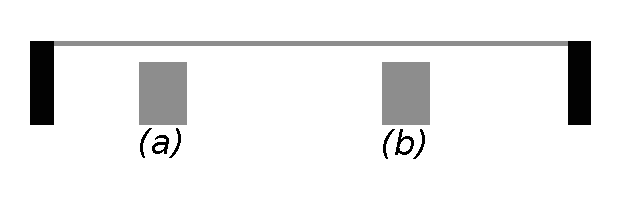
\includegraphics[width=0.7\textwidth]{images/setup}
\caption{Mock - just a template how to insert images.}
\label{fig:mock}
\end{figure}

\begin{figure}
\centering
\begin{minipage}{.47\linewidth}
\centering
\subfloat[]{\label{fig:prec:a}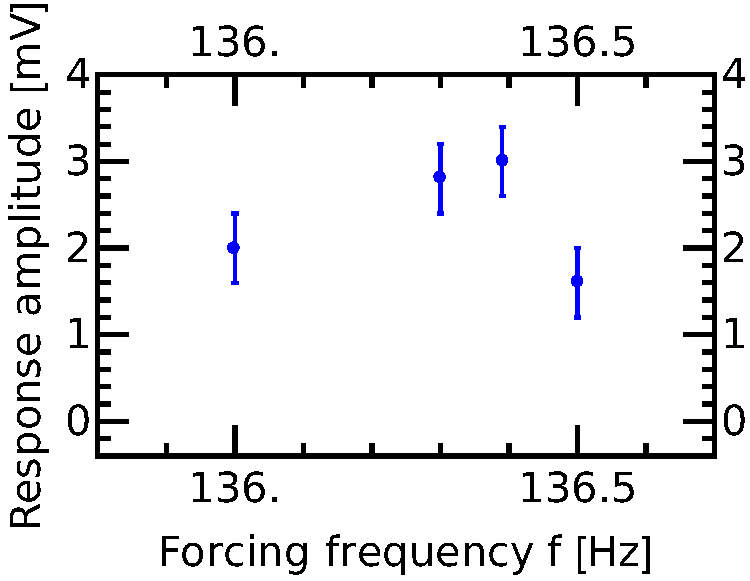
\includegraphics[width=\textwidth]{images/ampprec}}
\end{minipage}
\begin{minipage}{.47\linewidth}
\centering
\subfloat[]{\label{fig:prec:b}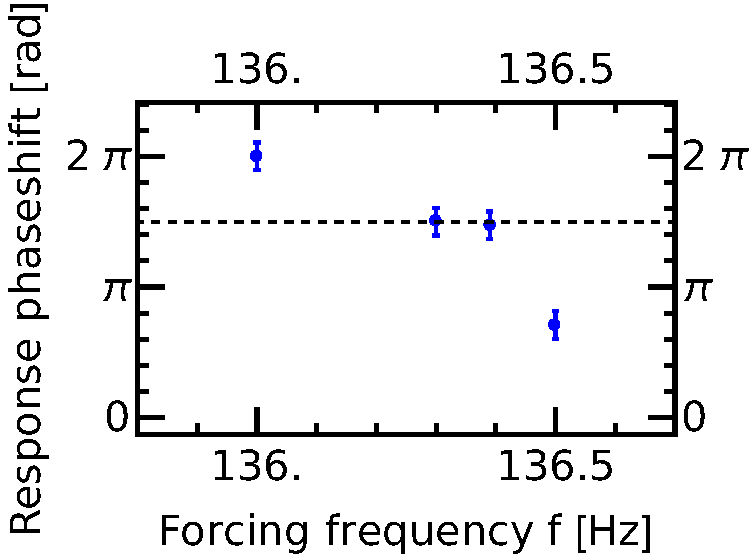
\includegraphics[width=\textwidth]{images/phaprec}}
\end{minipage}
\caption{Figure \ref{fig:prec:a} presents response amplitude as a function of frequency. Figure \ref{fig:prec:b} presents the phase-shift, dashed line denotes value $3\pi/4$ (value when the phase-shift is a quater of the whole period).
Both figures show that the resonance frequency can be estimated as 136.4(1) Hz.}
\label{fig:prec}
\end{figure}



\bibliographystyle{siam}
\bibliography{bibliography}
\end{document}
